% Standalone Orion invention-last router (Paper VI): SEARCH -> JUMP -> GLUE -> LIFT.
% Build:  pdflatex sjgl_router.tex  -> sjgl_router.pdf
\documentclass[border=6pt]{standalone}
\usepackage{tikz}
\usepackage{amsmath}
\usepackage{helvet}\renewcommand{\familydefault}{\sfdefault}
\usetikzlibrary{positioning,arrows.meta,shapes.geometric,fit,backgrounds,calc}
\definecolor{oiblue}{HTML}{0072B2}
\definecolor{oiverm}{HTML}{D55E00}
\definecolor{oigreen}{HTML}{009E73}
\begin{document}
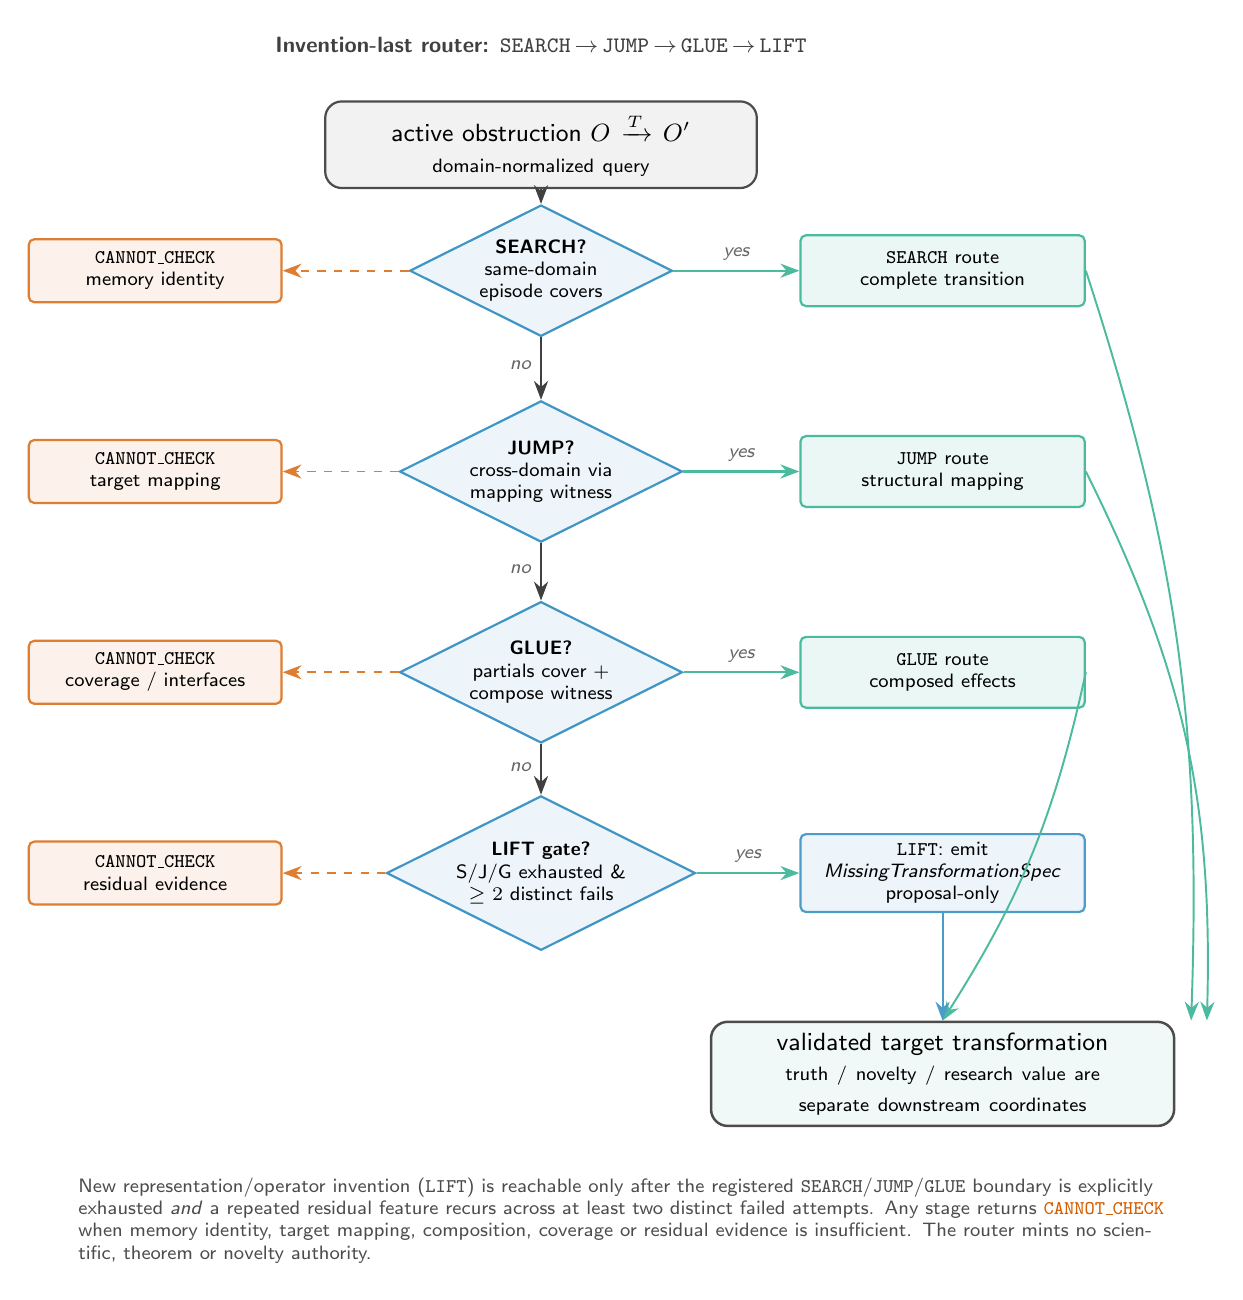
\begin{tikzpicture}[
  font=\small,
  >={Stealth[length=2.4mm]},
  startbox/.style={rounded corners=6pt, draw=black!70, line width=0.8pt, align=center,
                   inner sep=4pt, minimum height=11mm, text width=52mm, fill=black!5},
  dec/.style={diamond, aspect=2.0, draw=oiblue!75, line width=0.8pt, align=center,
              inner sep=1pt, fill=oiblue!7, font=\scriptsize},
  route/.style={rounded corners=2pt, draw=oigreen!70, line width=0.8pt, align=center,
                inner sep=3pt, minimum height=9mm, text width=34mm, fill=oigreen!8, font=\scriptsize},
  ccheck/.style={rounded corners=2pt, draw=oiverm!80, line width=0.8pt, align=center,
                 inner sep=3pt, minimum height=8mm, text width=30mm, fill=oiverm!8, font=\scriptsize},
  term/.style={rounded corners=6pt, draw=black!70, line width=0.9pt, align=center,
               inner sep=4pt, minimum height=10mm, text width=56mm, fill=oigreen!6},
  flow/.style={->, line width=0.7pt, draw=black!75},
  exitc/.style={->, line width=0.6pt, draw=oiverm!80, dashed},
  yes/.style={->, line width=0.8pt, draw=oigreen!70},
  lbl/.style={font=\scriptsize\itshape, text=black!60},
]
\def\ry{2.55}
% ---- start ----
\node[startbox] (start) at (0,1.6)
      {active obstruction $O\!\xrightarrow{T}\!O'$\\{\scriptsize domain-normalized query}};

% ---- decision spine (center) ----
\node[dec] (search) at (0,0)        {\textbf{SEARCH?}\\same-domain\\episode covers};
\node[dec] (jump)   at (0,-\ry)     {\textbf{JUMP?}\\cross-domain via\\mapping witness};
\node[dec] (glue)   at (0,-2*\ry)   {\textbf{GLUE?}\\partials cover +\\compose witness};
\node[dec] (lift)   at (0,-3*\ry)   {\textbf{LIFT gate?}\\S/J/G exhausted \&\\$\ge 2$ distinct fails};

% ---- success routes (right) ----
\node[route] (r1) at (5.1, 0)       {\texttt{SEARCH} route\\{\scriptsize complete transition}};
\node[route] (r2) at (5.1,-\ry)     {\texttt{JUMP} route\\{\scriptsize structural mapping}};
\node[route] (r3) at (5.1,-2*\ry)   {\texttt{GLUE} route\\{\scriptsize composed effects}};
\node[route, draw=oiblue!70, fill=oiblue!7] (r4) at (5.1,-3*\ry)
      {\texttt{LIFT}: emit\\\emph{MissingTransformationSpec}\\{\scriptsize proposal-only}};

% ---- CANNOT_CHECK exits (left) ----
\node[ccheck] (cc1) at (-4.9, 0)     {\texttt{CANNOT\_CHECK}\\{\scriptsize memory identity}};
\node[ccheck] (cc2) at (-4.9,-\ry)   {\texttt{CANNOT\_CHECK}\\{\scriptsize target mapping}};
\node[ccheck] (cc3) at (-4.9,-2*\ry) {\texttt{CANNOT\_CHECK}\\{\scriptsize coverage / interfaces}};
\node[ccheck] (cc4) at (-4.9,-3*\ry) {\texttt{CANNOT\_CHECK}\\{\scriptsize residual evidence}};

% ---- terminal ----
\node[term] (done) at (5.1,-4*\ry)
      {validated target transformation\\{\scriptsize truth / novelty / research value are separate downstream coordinates}};

% ---- edges: spine ----
\draw[flow] (start) -- (search);
\draw[flow] (search) -- node[lbl,left,pos=0.45]{no} (jump);
\draw[flow] (jump)   -- node[lbl,left,pos=0.45]{no} (glue);
\draw[flow] (glue)   -- node[lbl,left,pos=0.45]{no} (lift);

% ---- yes -> routes ----
\draw[yes] (search) -- node[lbl,above]{yes} (r1);
\draw[yes] (jump)   -- node[lbl,above]{yes} (r2);
\draw[yes] (glue)   -- node[lbl,above]{yes} (r3);
\draw[yes] (lift)   -- node[lbl,above]{yes} (r4);

% ---- CANNOT_CHECK exits ----
\foreach \d/\c in {search/cc1,jump/cc2,glue/cc3,lift/cc4}{
  \draw[exitc] (\d) -- (\c);
}

% ---- routes feed the validated transformation ----
\draw[flow, draw=oigreen!70] (r1.east) to[bend left=10] ([xshift=2mm]done.north east);
\draw[flow, draw=oigreen!70] (r2.east) to[bend left=14] ([xshift=4mm]done.north east);
\draw[flow, draw=oigreen!70] (r3.east) to[bend left=10] (done.north);
\draw[flow, draw=oiblue!70]  (r4) -- (done);

% ---- invention-last banner ----
\node[anchor=south, font=\footnotesize\bfseries, text=black!75] at (0,2.65)
      {Invention-last router: \texttt{SEARCH}\,$\rightarrow$\,\texttt{JUMP}\,$\rightarrow$\,\texttt{GLUE}\,$\rightarrow$\,\texttt{LIFT}};

% ---- note ----
\node[anchor=north west, font=\scriptsize, text width=140mm, align=left, black!70]
      at (-6.0,-4*\ry-1.2)
      {New representation/operator invention (\texttt{LIFT}) is reachable only after the registered
       \texttt{SEARCH}/\texttt{JUMP}/\texttt{GLUE} boundary is explicitly exhausted \emph{and} a repeated
       residual feature recurs across at least two distinct failed attempts. Any stage returns
       {\color{oiverm}\texttt{CANNOT\_CHECK}} when memory identity, target mapping, composition, coverage or
       residual evidence is insufficient. The router mints no scientific, theorem or novelty authority.};
\end{tikzpicture}
\end{document}
